\chapter{The Discontinuous Galerkin method}	\label{ch:NumericalMethods}
This chapter aims to give an overview of the basic ideas of the DG method, as well as to present the spatial and temporal discretization of the equations presented earlier. Parts of this chapter are based on the work presented at \parencite{kummerExtendedDiscontinuousGalerkin2017,kikkerFullyCoupledHighorder, smudamartinDirectNumericalSimulation2021}. The reader interested in a more in-depth description of the DG method is referred to the works of  \parencite{cockburnDevelopmentDiscontinuousGalerkin2000,hesthavenNodalDiscontinuousGalerkin2008,dipietroMathematicalAspectsDiscontinuous2012}

\section{State of the art}


\section{The Discontinuous Galerkin method}

\subsection{Definitions for the discretization} \label{ssec:SpatDiscretization}
First some standard definitions and notation are introduced in the context of DG methods. 

A computational domain $\Omega \subset \mathbb{R}^2$ with a polygonal and simply connected boundary $\partial \Omega$ is defined. The numerical grid is then formed by the set of non-overlapping elements $\gls{grid} = \{K_1, ..., K_J\}$ with a characteristic mesh size $h$, so that $\Omega$ is the union of all elements, i.e. $\Omega = \bigcup_{i=1}^J K_i$. 

Define $\Gamma = \bigcup_j \partial K_j$ as the union of all edges (internal edges and boundary edges) and $\Gamma_I = \Gamma \setminus \partial \Omega$ as the union of all interior edges.
For each edge of $\Gamma$ a normal field $\myvector{n}_{\Gamma}$ is defined. Particularly on $\partial \Omega$ the normal field is defined as an outer normal and $\vec{n}_\Gamma = \vec{n}_{\partial\Omega}$.
For each field ${u} \in C^0\left(\Omega\setminus \Gamma_I\right)$, ${u}^-$  and ${u}^+$ is defined, which describe the values of the variables on the interior and exterior sides of the cell:
\begin{align}
	{u}^- & = \lim_{\xi \searrow 0} {u}\left(\myvector{x} - \xi \myvector{n}_{\Gamma}\right) \quad \text{for } \myvector{x}\in \Gamma   \\
	{u}^+ & = \lim_{\xi \searrow 0} {u}\left(\myvector{x} + \xi \myvector{n}_{\Gamma}\right) \quad \text{for } \myvector{x}\in \Gamma_I
\end{align}
The jump and mean values of ${u}$ on the inner edges $\Gamma_I$ are defined as
\begin{align}
	\llbracket {u} \rrbracket & = {u}^+-{u}^-                           \\
	\{{u}\}                   & = \frac{1}{2} \left({u}^-+{u}^+\right).
\end{align}
while the jump and mean values on the boundary edges $\partial \Omega$ are:
\begin{align}
	\llbracket {u} \rrbracket & = {u}^-  \\
	\{{u}\}                   & = {u}^-.
\end{align}
Furthermore, the broken polynomial space of a total degree $k$ is defined as
\begin{equation}
	\mathbb{P}_k(\gls{grid} )= \{f \in L^2\left(\Omega\right); \forall K \in \gls{grid} : f\vert_{K} \text{ is polynomial and deg}\left(f\vert_{K}\right)\leq k \}.
	\label{Eq:PolSpace}
\end{equation}
Additionally, for $u \in \mathcal{C}^1(\Omega \setminus \Gamma)$ the broken gradient $\nabla_h u$ is defined as:
\begin{equation}
	\nabla_h u
	= \begin{cases}
		0
		 & \text{on }\Gamma  \\
		\nabla u
		 & \text{elsewhere }
	\end{cases}
\end{equation}
The broken divergence $\nabla_h \cdot u$ is defined analogously. Furthermore, the function space for test and trial functions for $D_v$ dependent variables is defined as
\begin{equation}
	\mathbb{V}_\myvector{k} = \prod_{i=1}^{D_v} \mathbb{P}_{k_i}(K_h)
	\label{Eq:Vspace}
\end{equation}
where $\myvector{k} = \left(k_1,...,k_{D_v}\right)$. 
Additionally, for a cell $K$ we define for $u_K$, $v_K\in \mathbb{V}_\myvector{k}$ a local inner product and a local $L^2$-norm as
\begin{equation}
(u_K, v_K)_K \coloneqq \int_K u_K v_K\text{d}x, \qquad \norm{u_K}^2_K \coloneqq(u_K,u_K)_K
\end{equation}
Similarly, for $u_h$, $v_h \in \mathbb{V}_\myvector{k}$ a global inner product and global broken norm are defined as
\begin{equation}
	(u_h, v_h)_{\Omega_h} \coloneqq \sum_{i = 1}^N (u_h, v_h)_K, \qquad \norm{u_h}^2_{\Omega_h} \coloneqq(u_h,u_h)_{\Omega_h}
\end{equation}
\subsection{Discretization using the DG Method} \label{sec:DiscWithDG}
In this subsection the discretization of a simple problem using the DG method will be shown in order to demonstrate how it works and some of its specific characteristics. For this purpose, the discretization of a general conservation law for a scalar quantity $u = u(\vec{x},t)$ governed by a nonlinear flux function $\vec{f}(u)$ will be considered. In addition, suitable Dirichlet boundary conditions on $\partial \Omega = \partial \Omega_D$ and initial conditions $u_0$ are defined. The problem reads
\begin{subequations}
\begin{align}
&\pfrac{u}{t} + \nabla \cdot \vec{f}(u) = 0, \qquad\qquad\qquad &\vec{x} \in \Omega,\label{eq:consEqDG}\\
&u = u_D, \qquad \qquad \qquad  &\vec{x} \in \partial \Omega_D,\\
&u(\vec{x},0) = u_0(\vec{x}), \qquad\qquad\qquad &\vec{x}\in\Omega.
\end{align}\label{eqs:DGTransportExample}
\end{subequations}
The DG-method allows finding an approximate solution $u_h = u_h(\vec{x},t)$ for the problem defined by \cref{eqs:DGTransportExample} by forming a linear combination of polynomial functions in each cell.  The discretization procedure starts by the approximation of the domain $\gls{domain}$ with a numerical grid $\gls{grid}$. In each cell $K_j$ of the numerical grid a set of polynomial basis $\vectr{\phi}_j = (\tilde{\phi}_{j,l})_{l=1,\dots,N_k} \in \mathbb{P}_k(\mathcal{K}_h)$ with a local cell support $\text{supp}(\phi_j) = \overline{\gls{cell}}_j$ is defined. This allows to represent the local solution for each cell $K_j$ as
\begin{equation}
u_j(\vec{x},t) = \sum_{l=1}^{N_k}\tilde{u}_{j,l}(t)\phi_{j,l}(\vec{x}) = \tilde{\vec{u}}_j(t) \cdot \vectr{\phi}_j (\vec{x})\label{eq:DGAnsatz}
\end{equation}
The coefficients $\tilde{\vectr{u}}_j = (\tilde{u}_{j,l})_{l=1,\dots,N_k}$ are the \gls{DOFs} of the local solution in the cell $K_j$, which are the unknowns of the problem. Note the time dependence of the coefficients $\tilde{\vec{u}}_j$, as well as the dependence of the basis functions $\vectr{\phi}_j (\vec{x})$ on the vector $\vec{x}$. 

This approximate solution sought  is the best approximation of $\gls{DGVar} \in L^2(\gls{domain})$, which gives a minimum global error in the approximation space $\gls{DGVar} \in \mathbb{P}_k(\gls{domain} )$. 
\begin{align}
	\int_{\domain} (\underbrace{ \nuM{\gls{DGVar}}(x)-\gls{DGVar}(x) }_{=: \gls{dgerror}(x)})^2 \dV
	= ||\nuM{\gls{DGVar}} - \gls{DGVar}||_2^2 \rightarrow \text{min}
\end{align}
Here $\gls{dgerror}$ is the error of the discretization. Minimization is equivalent to requiring
\begin{equation}
	\label{eq:L2projection}
	\scp{r(x)}{\basis{}_m} = \scp{f_h-f}{\basis{}_m} \stackrel{!}{=} 0 \qquad \forall\basis{}_m
\end{equation}
This means that the error is orthogonal to every polynomial function $ \basis{}_m$ in the approximation space. The Bramble-Hilbert lemma \parencite{brambleEstimationLinearFunctionals1970} says, that for a $p$-times differentiable variable $\gls{DGVar}$, the error is of the order $\mathcal{O}(h^{p+1})$, which is one of the major motivations for the use of high order methods. The differentiability assumption is essential. For non smooth $\gls{DGVar}$ the well known Gibbs phenomenon occurs.

There are two general approaches used for the representation of the solution using basis functions: modal and nodal. Each one of them present some advantages and disadvantages \parencite{hesthavenNodalDiscontinuousGalerkin2008}. In this work, a modal polynomial representation is used. The basis functions are chosen such that they are orthogonal to each other 
\begin{equation}
	\int_{K_j} \phi_{j,m}\phi_{j,n} \text{d}V= \delta_{mn}
\end{equation}
where $\delta_{mn}$ is the Kronecker delta. In the present work Legendre polynomials are used, since they present the orthogonality property. This property implies that the mass matrix (to be defined later) equals the identity matrix.

By inserting the approximate solution defined by \cref{eq:DGAnsatz} in the conservation \cref{eq:consEqDG}, a local residual $R_j$ can be defined
\begin{equation}\label{eq:DGResidualeq}
R_j(\vec{x},t) = \pfrac{u_j}{t} + \nabla \cdot \vec{f}(u_j), \quad \vec{x} \in K_j
\end{equation}
Minimization of this local residual is done by multiplying \cref{eq:DGResidualeq} by the so called tests functions. In the Galerkin approach, these test functions are required to be from the same space as the trial functions, i.e. $\gls{testF}_{j,l} = \gls{basis}_{j,l}$. Thus, by multiplying \cref{eq:DGResidualeq} by a trial function and integrating over the cell $K_j$, one obtains
\begin{equation}
	\int_{\gls{cell}_j} \gls{DGres}_j \gls{testF}_{j,l} \d{V} = \int_{\gls{cell}_j}  \pDeriv{{\gls{DGVar}}_j}{t} \gls{basis}_{j,l} + \div{\gls{flux}({\gls{DGVar}}_j)} \gls{basis}_{j,l} \d{V} \stackrel{!}{=} 0, \quad \forall \vectr{\gls{basis}}_{j,l}.
	\label{eq:DGminimization}
\end{equation}
Where the minimization comes from requiring the equality to zero. Note that until this point only a cell-local discretization has been addressed. The next step for obtaining a global DG formulation is to use integration by parts for rewriting the spatial term in \cref{eq:DGminimization}. This is done to make the boundary edge integrals explicitly appear in the formulation, which are used later to couple cell $K_j$ with neighbouring cells. The partial integration process results in
 \begin{equation}
	\int_{\gls{cell}_j}  \pDeriv{{\gls{DGVar}}_j}{t} \gls{basis}_{j,l} \d{V} + \oint_{\partial{\gls{cell}}_j} \left( \gls{flux}({\gls{DGVar}}_j)\cdot{\gls{normal}}_j \right) \gls{basis}_{j,l} \d{S} - \int_{\gls{cell}_j} \gls{flux}({\gls{DGVar}}_j) \cdot \gradH{\gls{basis}}_{j,l} \d{V}  = 0, \quad \forall \gls{basis}_{j,l},
	\label{eq:DGfluxFormulation}
\end{equation} 
Note that inserting the ansatz \cref{eq:DGAnsatz} into \cref{eq:DGfluxFormulation} is problematic, since $\partial{\gls{cell}}_j$ is shared by other cells, and in the DG method continuity of a variable is not enforced across cell boundaries. This means that in general the inner value $u^{-}_j$ and the outer value $u^{+}_j$ are not equal. This problem is solved by introducing the concept of a numerical flux function, denoted here with $\gls{numflux}$
\begin{equation}
	\gls{numflux}(\inn{{\gls{DGVar}}_j}, \out{{\gls{DGVar}}_j}, \gls{normalGam}) \approx \gls{flux}({\gls{DGVar}}_j) \cdot {\gls{normal}}_j.
\end{equation}
This expression defines an unique value for the flux of a given cell boundary, enforcing flux continuity. The numerical flux $\gls{numflux}$ couples the \gls{DOFs} of neighbouring cells, and should satisfy certain mathematical and physical properties which will be discussed later. Many different numerical fluxes have been developed, and it is an active area of investigation. They differ mainly in computational cost, stability and dissipation of the scheme.

By introducing the numerical flux in \cref{eq:DGfluxFormulation} the problem now reads
\begin{equation}
	\int_{\gls{cell}_j}  \pDeriv{{\gls{DGVar}}_j}{t} \gls{basis}_{j,l} \d{V} + \oint_{\partial{\gls{cell}}_j} \left( \gls{numflux}(\inn{{\gls{DGVar}}_j}, \out{{\gls{DGVar}}_j}, \gls{normalGam})    \right) \gls{basis}_{j,l} \d{S} - \int_{\gls{cell}_j} \gls{flux}({\gls{DGVar}}_j) \cdot \gradH{\gls{basis}}_{j,l} \d{V}  = 0, \quad \forall \gls{basis}_{j,l},
	\label{eq:DGNumericalfluxFormulation}
\end{equation} 
\subsubsection{The global formulation}
Note that \cref{eq:DGNumericalfluxFormulation} is still a local formulation. A global solution $u(\vec{x},t)$ can be defined by a piecewise polynomial approximation according to 
\begin{equation}
	u(\vectr{x},t) \approx  u_h(\vectr{x},t) = \bigoplus\limits_{j=1}^{J} {\gls{DGVar}}_j(\vectr{x},t) = \sum_{j=1}^{J} \sum_{l=1}^{\gls{NoDOFloc}} \tilde{\gls{DGVar}}_{j,l}(t) \gls{basis}_{j,l}(\vectr{x}) \in \gls{brknPspacek}(\gls{grid})
	\label{eq:globalApprox}
\end{equation}
which corresponds to the direct sum of the $J$ local solutions $u_j$. A vector $\tilde{\vec{u}} = \tilde{\gls{DGVar}}_{1,1},\allowbreak \tilde{\gls{DGVar}}_{1,2},\allowbreak\dots, \allowbreak \tilde{\gls{DGVar}}_{j,l},\allowbreak\dots,\allowbreak\tilde{\gls{DGVar}}_{J,\gls{NoDOFloc}}\allowbreak$ which comprises all the DOFs of the global approximation $\gls{DGVar}_h$ is defined, and is of length $\gls{NoDOF} = J\cdot\gls{NoDOFloc}$.%

Finally, the global formulation is obtained by inserting the ansatz \cref{eq:DGAnsatz} into \cref{eq:DGNumericalfluxFormulation}, summing over all cells $K_j$ and making use of \cref{eq:globalApprox}. The problem reads: Find $\nuM{\gls{DGVar}} \in 	\mathbb{P}_k(\gls{grid})$, such that $\forall \phi \in 	\mathbb{P}_k(\gls{grid})$
\begin{equation}
	\int_{\gls{domain}}  \pDeriv{\nuM{\gls{DGVar}}}{t} \gls{basis} \d{V}  + \oint_{\gls{edge}} \gls{numflux}(\inn{\nuM{\gls{DGVar}}}, \out{\nuM{\gls{DGVar}}}, \gls{normalGam}) \jump{\gls{basis}} \d{S} - \int_{\gls{domain}} \gls{flux}(\nuM{\gls{DGVar}}) \cdot \gradH{\gls{basis}} \d{V} = 0,
	\label{eq:semiDiscWeakForm}
\end{equation}
The solution of this system requires finding the DOFs $\tilde{\vec{u}}$ of the global approximation $\gls{DGVar}_h$. Dirichlet boundary conditions are included in the formulation by defining at $\gls{edge}_D$ the outer value $\out{\gls{DGVar}}_h = \gls{DGVar}_D$.

Note that \cref{eq:semiDiscWeakForm} is semi-discrete, meaning that the system of equations has been discretized in space, but not in time. Time discretization will be treated in \cref{ssec:TemporalDiscretization}.

Finally, after selecting suitable numerical fluxes for the various terms of the governing equations, a system is obtained that in general has the form
%\begin{equation}
%	 \deriv{ }{t} \left( {\gls{massM}}(\tilde{\vectr{\gls{DGVar}}})\tilde{\vectr{\gls{DGVar}}} \right) + \gls{OpM}(\tilde{\vectr{\gls{DGVar}}}) = \vectr{b},
%	\label{eq:discretMatrixForm}
%\end{equation}
\begin{equation}
	 \deriv{ \tilde{\vectr{\gls{DGVar}}}}{t}+ \gls{OpM}(\tilde{\vectr{\gls{DGVar}}}) = \vectr{b},
	\label{eq:discretMatrixForm}
\end{equation}
Where $\gls{massM}$ is the mass matrix, and $\gls{OpM}$ is the operator matrix.  The vector $b$ contains the Dirichlet boundary condition. The operator matrix is defined locally by
\begin{equation}
	(\gls{OpM}_j)_{m,n} =  \oint_{\partial{\gls{cell}}_j} \gls{numflux}(\tilde{{\gls{DGVar}}}_{j,n}, \tilde{{\gls{DGVar}}}_{j^{\ast},n},\gls{normalI}) \gls{basis}_{j,m} \d{S} - \int_{\gls{cell}_j} \gls{flux}(\tilde{{\gls{DGVar}}}_{j,n} {\gls{basis}}_{j,n}) \cdot \gradH{\gls{basis}}_{j,m} \d{V} ,
	\label{eq:genOpMatrix}
\end{equation}
with $j^{\ast}$ denoting the index of a neighbour cell. The matrix $\gls{OpM}$ has block-diagonal structure, but also including extra diagonals which relate the DOFs of the cell with the neighbouring cells.

The global mass matrix is
\begin{equation}
	{\gls{massM}} =
	\left[ 
	\begin{array}{cccc}
		{\gls{massM}}_{1} & 0 & \cdots & 0 \\
		0 & {\gls{massM}}_{2} & \cdots & 0 \\
		\vdots & \vdots & \ddots & \vdots \\
		0 & 0 & \cdots & {\gls{massM}}_{J}
	\end{array}
	\right],
\end{equation} 
which is block-diagonal, since  ${\gls{massM}}_{j}$ does not depend on neighbouring cells. 
\begin{equation}
	({\gls{massM}}_j)_{m,n} = \int_{\gls{cell}_j} \gls{basis}_{j,m} \gls{basis}_{j,n} \d{V}	\label{eq:massMatrix}
\end{equation} 
The mass matrix of a cell ${\gls{massM}}_{j} := \matrixDG{M}_{(j,-) \ (j,-)} $ only depends in this case on the cell-local basis functions. 
%\todo[inline]{How is the mass matrix defined for variable density flows?}

\subsubsection{Note on the numerical fluxes}
As mentioned before, the numerical fluxes $\gls{numflux}$ have to fulfil certain physical and mathematical properties for obtaining a stable and convergent method. One of the requirement for proving the stability of the scheme is the monotonicity. First, the energy estimate is defined as
\begin{equation}
	\norm{\gls{DGVar}(\vectr{x},t)}_{\gls{domain}}^2 \leq \norm{\gls{DGVar}(\vectr{x},0)}_{\gls{domain}}^2, \quad \forall t \geq 0,
	\label{eq:energyEstimate}
\end{equation}
assuming homogeneous Dirichlet boundary conditions. This means that the system is stable if the energy norm $\norm{\gls{DGVar}(\vectr{x},t)}_{\gls{domain}}^2 $ is strictly decreasing in the absence of inflow. 

For a monotonic numerical flux is possible to show that the discrete problem \cref{eq:semiDiscWeakForm} satisfies the discrete equivalent of \cref{eq:energyEstimate}. In addition to the monotonicity of the numerical flux, it is necessary that $\gls{numflux}$ is Lipschitz continuous.%, which means
%\begin{equation}
%	\label{eq:flux_lipschitz_first}
%	\exists C_a \in \mathbb{R}: \abs{\gls{numflux}(a_1, b, \vec{n}) - \hat{f}(a_2, b, \vec{n})} \leq C_a \abs{a_1 - a_2} 
%	\qquad \forall a_1, a_2 \in \mathbb{R}
%\end{equation}
%and
%\begin{equation}
%	\label{eq:flux_lipschitz_second}
%	\exists C_b \in \mathbb{R}: \abs{\gls{numflux}(a, b_1, \vec{n}) - \hat{f}(a, b_2, \vec{n})} \leq C_b \abs{b_1 - b_2} 
%	\qquad \forall b_1, b_2 \in \mathbb{R}
%\end{equation}
For the complete proof the interested reader is referred to the book from \textcite{dipietroMathematicalAspectsDiscontinuous2012}.

Two more requirements are needed for the numerical flux. The first is the consistency of the flux, which can be written as
\begin{equation}
	\gls{numflux}(a,a,\gls{normal}) = \gls{flux}(a) \cdot \gls{normal}, \quad \forall a \in \mathbb{R}. 
	\label{eq:consistency}
\end{equation}
showing that a numerical flux function should deliver the same approximate solution that the original flux function in case of a continuous variable across the interface. A direct consequence of the consistency of the numerical flux is that the weak formulation \cref{eq:semiDiscWeakForm} is automatically fulfilled by $\nuM{\gls{DGVar}} = \gls{DGVar}$.

Finally the last requirement is that the numerical flux should be conservative, which means that the total amount of $\gls{DGVar}$ can only change due to fluxes across the domain boundary. This can be written as
\begin{equation}
	\gls{numflux}(a,b,\gls{normal}) = 	-\gls{numflux}(b,a,-\gls{normal}), \quad \forall a,b \in \mathbb{R}. 
	\label{eq:conservativity}
\end{equation}
All numerical fluxes used in this work for the spatial discretization of \cref{eq:all-eqs} fulfil these requirements and they will be shown in the next section.
\subsection{Temporal discretization}\label{ssec:TemporalDiscretization}
This section will give a brief introduction to the most popular time-stepping techniques and then show the time-stepping method used in this work. This section is mainly based on \textcite{levequeFiniteVolumeMethods2002,ferzigerComputationalMethodsFluid2002}.
%\subsubsection{}
In the previous chapter the spatial discretization using a DG method was shown, resulting in the semi-discrete formulation given by \cref{eq:semiDiscWeakForm}. The time discretization of this semi-discrete system leads to the so called method of lines, which is the name for a method first discretized in space, and later in time.  

An alternative to the method of lines is the so called Rothe's method, where time is first discretized then the space. This can be advantageous in some cases, such as problems with a moving domain. Another alternative is the space-time approach, where basically the temporal coordinate is treated as another spatial dimension. Again, the method can be very attractive for some cases. However, the discretized schemes lead often to prohibitively large systems. These approaches are ignored in the present work, and the method of lines is adopted.

First the time discretization for a system with a constant mass matrix will be discussed. The process of discretization results often in a system of ordinary differential equations (ODEs) of the form
\begin{equation}
\gls{massM}\frac{\text{d}\vec{u}}{\text{d}t} = - \vec{F}(t,\vec{u}(t))\qquad \text{for}\qquad t \in (0,T).\label{eq:timestep1}
\end{equation}
with a initial condition given by $\vec{u}(t=0) = \vec{u}^0$. The main idea of a time-stepper algorithm is to discretize the time coordinate, and advance gradually the solution $\vec{u}(t^n)$ in time from values at previous time levels $\vec{u}(t^{n-1})$, $\vec{u}(t^{n-2})$, $\dots$,  until a certain final time $t = T$ is reached.
By integrating \cref{eq:timestep1} in time, one obtains
\begin{equation}
\gls{massM}(\vec{u}(t^{n+1})-\vec{u}(t^{n})) = - \int_{t^n}^{t^{n+1}}\vec{F}(t,\vec{u}(t)) \text{d}t \label{eq:timestep2}
\end{equation}
This equation is the starting point for different class of time stepping techniques. Two kind of methods can be distinguished, depending on how the integral in \cref{eq:timestep2} is evaluated: explicit methods and explicit methods. Explicit methods are obtained when the approximation of the integral is done only by using information from old time steps, while for implicit methods the information from the actual timestep is also considered, making necessary the solution of a system of equations.

The simplest example of an explicit time-stepping method is the Explicit Euler Method:
\begin{equation}
\gls{massM}\vec{u}(t^{n+1})= \gls{massM}\vec{u}(t^{n})  - \Delta t \vec{F}(t^n,\vec{u}(t^n)),
\end{equation}
which is first order accurate in time. Other explicit methods exists with better properties than the Explicit Euler Method, typically using information from multiple known time levels or a interpolation of them. Adams-Bashforth methods are a good exponent of them. 

Due to the local nature of the approach, explicit methods present themselves specially attractive for DG methods, particularly for hyperbolic equations. Explicit methods are relatively easy to implement, and need considerably less storage compared to implicit methods. However, explicit methods experience the disadvantage that the stability of the algorithm is heavily limited by a maximal timestep size $\Delta t$. The timestep typically scales with the grid size $h$ and polynomial degree $k$ by $\Delta \sim h/k$ for hyperbolic and $\Delta \sim (h/k)^2$ for parabolic problems \parencite{gassnerContributionConstructionDiffusion2007}. For many problems of interest, particularly stiff systems, this limitation is highly restrictive, since very little timesteps need to be chosen in order to obtain a stable method. 

Implicit methods  on the other hand are specially well suited for stiff problems, as they don't suffer from the restrictive timestep limitation of explicit methods, even not being restricted at all under certain conditions. This allows using considerably bigger timesteps. Implicit methods present however the inconvenience that they require the solution of a system of equations, which for large problems is not a trivial task and specialized methods are needed. The use of implicit methods is justified, particularly for stiff problems, as the extra computational overhead originating from the resolution of the system of equations is usually smaller than the time it would take to solve the same problem using explicit schemes with very small timesteps.

The simplest implicit method is the Implicit Euler Method 
\begin{equation}
\gls{massM}\vec{u}(t^{n+1}) + \Delta t\vec{F}(t^{n+1},\vec{u}(t^{n+1}))= \gls{massM}\vec{u}(t^{n})  
\end{equation}
Note that this is a non-linear system of algebraic equations that has to be solved for $\vec{u}(t^{n+1})$ iteratively. The Implicit Euler Methods is the first method of a family of backward differentiation formulas (BDF), and presents the property of being unconditionally stable, meaning that the algorithm allows an arbitrarily large timestep. This property allows the calculation of steady state solutions just by choosing a very big $\Delta t$ value. However, not all BDF schemes are unconditionally stable, as it will be shown next.
\subsubsection{Backward Differentiation Formula}
\begin{table}[b]
	\centering
	\begin{tabular}{lllllll}
		\hline
		$s$                   & $\gamma$ & $\beta_0$ & $\beta_1$ & $\beta_2$ & $\beta_3$ & $\beta_4$ \\ \hline
		Implicit Euler (BDF1) & 1        & 1         & -1        &           &           &           \\
		BDF2                  & 2        & 3         & -4        & 1         &           &           \\
		BDF3                  & 6        & 11        & -18       & 9         & -2        &           \\
		BDF4                  & 12       & 25        & -48       & 36        & -16       & 3         \\ \hline
	\end{tabular}
	\caption{Coefficients of the BDF schemes.}
	\label{tab:BDFCoeff}
\end{table}
In the present work BDF methods are used. In case of a non-constant mass matrix $\gls{massM}$, they have a general formula given by
\begin{equation}
	\frac{\beta_0}{\gamma\Delta t}\gls{massM}(\vec{u}(t^n))\vec{u}(t^n)- \vec{F}(\vec{u}(t^n)) = - \sum_{i=1}^s \frac{\beta_i}{\gamma \Delta t}\gls{massM}(\vec{u}(t^{n-i}))\vec{u}(t^{n-i}).
\end{equation}\label{eq:BDFDiscretization}
where $s$ is the order of the BDF-scheme.  The coefficients of each schema are shown in \cref{tab:BDFCoeff}. The main advantage of BDF methods is their large stability regions, which make them suitable for solving stiff problems.  In \cref{Fig:AStability} the stability regions for the first four BDF schemes are shown. It is possible to observe that only the BDF-1 (implicit Euler) and BDF-2 schemes exhibit the property that they are A-stable, which means that the stability region contains the entire left complex plane \parencite{dahlquistSpecialStabilityProblem1963}. On the other hand, BDF schemes of order $s > 2$ are not A-stable. In this work however, BDF schemes up to order three have been used, as the unstable eigenvalues for $z=3$ are comparatively small \parencite{smudamartinDirectNumericalSimulation2021}.
The solution of problems of the form of \cref{eq:BDFDiscretization} will be treated in \cref{sec:CompMethodology}.

\begin{figure}
	\centering
	\pgfplotsset{width=0.5\textwidth}
	% This file was created by matlab2tikz.
%
%The latest updates can be retrieved from
%  http://www.mathworks.com/matlabcentral/fileexchange/22022-matlab2tikz-matlab2tikz
%where you can also make suggestions and rate matlab2tikz.
%
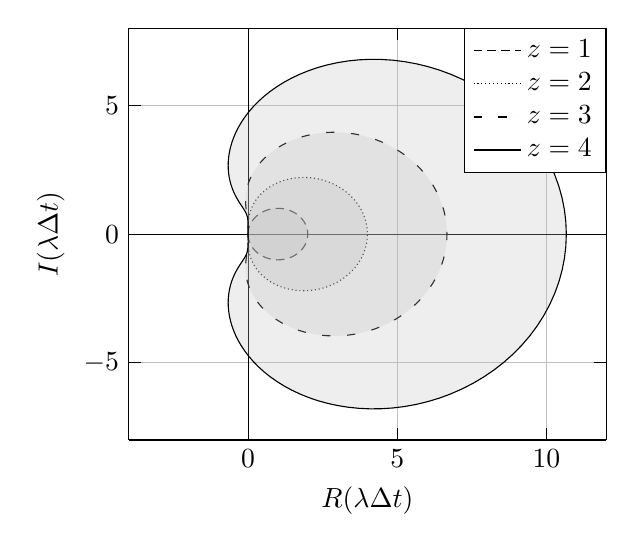
\begin{tikzpicture}	
	\begin{axis}[%
%		width=3.566in,
%		height=3.566in,
		at={(1.236in,0.481in)},
		scale only axis,
		separate axis lines,
		every outer x axis line/.append style={black},
		every x tick label/.append style={font=\color{black}},
		every x tick/.append style={black},
		xmin=-4,
		xmax=12,
		every outer y axis line/.append style={black},
		every y tick label/.append style={font=\color{black}},
		every y tick/.append style={black},
		ymin=-8,
		ymax=8,
		axis background/.style={fill=white},
		xlabel=$\mathfrak{R}(\lambda \Delta t)$,
		ylabel=$\mathfrak{I}(\lambda \Delta t)$,
		xmajorgrids,
		ymajorgrids,
		legend style={at={(1,1)}, anchor=north east},
		]
		\addplot [color=black, forget plot]
		table[row sep=crcr]{%
			-40	0\\
			40	0\\
		};
		\addplot [color=black, forget plot]
		table[row sep=crcr]{%
			0	-40\\
			0	40\\
		};
		\addplot [color=black, fill=lightgray, fill opacity=0.25, densely dashed]
		table[row sep=crcr]{%
			0	0\\
			0.000493439634268511	0.0314107590781283\\
			0.00197327157172855	0.0627905195293134\\
			0.00443803539692	0.0941083133185143\\
			0.00788529868552224	0.125333233564304\\
			0.0123116594048625	0.156434465040231\\
			0.0177127492713113	0.187381314585725\\
			0.0240832380612526	0.218143241396543\\
			0.0314168388713688	0.248689887164855\\
			0.039706314323057	0.278991106039229\\
			0.0489434837048464	0.309016994374947\\
			0.0591192310457745	0.338737920245291\\
			0.0702235141117485	0.368124552684678\\
			0.0822453743160189	0.397147890634781\\
			0.0951729475339805	0.425779291565073\\
			0.108993475811632	0.453990499739547\\
			0.123693319956137	0.481753674101715\\
			0.139257972996056	0.509041415750371\\
			0.155672074497985	0.535826794978997\\
			0.172919425725438	0.562083377852131\\
			0.190983005625053	0.587785252292473\\
			0.20984498762431	0.612907053652976\\
			0.229486757224211	0.63742398974869\\
			0.24988893036954	0.661311865323652\\
			0.271031372578588	0.684547105928689\\
			0.292893218813452	0.707106781186547\\
			0.315452894071311	0.728968627421411\\
			0.338688134676348	0.750111069630459\\
			0.36257601025131	0.770513242775789\\
			0.387092946347024	0.79015501237569\\
			0.412214747707527	0.809016994374947\\
			0.437916622147869	0.827080574274562\\
			0.464173205021003	0.844327925502015\\
			0.490958584249629	0.860742027003944\\
			0.518246325898285	0.876306680043864\\
			0.546009500260453	0.891006524188368\\
			0.574220708434927	0.904827052466019\\
			0.602852109365219	0.917754625683981\\
			0.631875447315322	0.929776485888251\\
			0.661262079754709	0.940880768954225\\
			0.690983005625053	0.951056516295154\\
			0.721008893960771	0.960293685676943\\
			0.751310112835145	0.968583161128631\\
			0.781856758603457	0.975916761938747\\
			0.812618685414275	0.982287250728689\\
			0.843565534959769	0.987688340595138\\
			0.874666766435696	0.992114701314478\\
			0.905891686681486	0.99556196460308\\
			0.937209480470687	0.998026728428271\\
			0.968589240921872	0.999506560365731\\
			1	1\\
			1.03141075907813	0.999506560365731\\
			1.06279051952931	0.998026728428271\\
			1.09410831331851	0.99556196460308\\
			1.1253332335643	0.992114701314478\\
			1.15643446504023	0.987688340595138\\
			1.18738131458572	0.982287250728689\\
			1.21814324139654	0.975916761938747\\
			1.24868988716485	0.968583161128631\\
			1.27899110603923	0.960293685676943\\
			1.30901699437495	0.951056516295154\\
			1.33873792024529	0.940880768954225\\
			1.36812455268468	0.929776485888251\\
			1.39714789063478	0.917754625683981\\
			1.42577929156507	0.90482705246602\\
			1.45399049973955	0.891006524188368\\
			1.48175367410172	0.876306680043863\\
			1.50904141575037	0.860742027003944\\
			1.535826794979	0.844327925502015\\
			1.56208337785213	0.827080574274562\\
			1.58778525229247	0.809016994374947\\
			1.61290705365298	0.79015501237569\\
			1.63742398974869	0.770513242775789\\
			1.66131186532365	0.75011106963046\\
			1.68454710592869	0.728968627421411\\
			1.70710678118655	0.707106781186548\\
			1.72896862742141	0.684547105928689\\
			1.75011106963046	0.661311865323652\\
			1.77051324277579	0.63742398974869\\
			1.79015501237569	0.612907053652976\\
			1.80901699437495	0.587785252292473\\
			1.82708057427456	0.562083377852131\\
			1.84432792550201	0.535826794978997\\
			1.86074202700394	0.509041415750371\\
			1.87630668004386	0.481753674101715\\
			1.89100652418837	0.453990499739547\\
			1.90482705246602	0.425779291565073\\
			1.91775462568398	0.397147890634781\\
			1.92977648588825	0.368124552684678\\
			1.94088076895423	0.338737920245291\\
			1.95105651629515	0.309016994374948\\
			1.96029368567694	0.27899110603923\\
			1.96858316112863	0.248689887164855\\
			1.97591676193875	0.218143241396543\\
			1.98228725072869	0.187381314585725\\
			1.98768834059514	0.156434465040231\\
			1.99211470131448	0.125333233564305\\
			1.99556196460308	0.0941083133185144\\
			1.99802672842827	0.0627905195293136\\
			1.99950656036573	0.0314107590781282\\
			2	1.22464679914735e-016\\
			1.99950656036573	-0.031410759078128\\
			1.99802672842827	-0.0627905195293133\\
			1.99556196460308	-0.0941083133185141\\
			1.99211470131448	-0.125333233564304\\
			1.98768834059514	-0.156434465040231\\
			1.98228725072869	-0.187381314585725\\
			1.97591676193875	-0.218143241396543\\
			1.96858316112863	-0.248689887164855\\
			1.96029368567694	-0.278991106039229\\
			1.95105651629515	-0.309016994374947\\
			1.94088076895423	-0.338737920245291\\
			1.92977648588825	-0.368124552684678\\
			1.91775462568398	-0.39714789063478\\
			1.90482705246602	-0.425779291565072\\
			1.89100652418837	-0.453990499739547\\
			1.87630668004386	-0.481753674101715\\
			1.86074202700394	-0.509041415750371\\
			1.84432792550202	-0.535826794978997\\
			1.82708057427456	-0.56208337785213\\
			1.80901699437495	-0.587785252292473\\
			1.79015501237569	-0.612907053652977\\
			1.77051324277579	-0.63742398974869\\
			1.75011106963046	-0.661311865323652\\
			1.72896862742141	-0.684547105928688\\
			1.70710678118655	-0.707106781186547\\
			1.68454710592869	-0.728968627421412\\
			1.66131186532365	-0.750111069630459\\
			1.63742398974869	-0.770513242775789\\
			1.61290705365298	-0.79015501237569\\
			1.58778525229247	-0.809016994374947\\
			1.56208337785213	-0.827080574274562\\
			1.535826794979	-0.844327925502015\\
			1.50904141575037	-0.860742027003944\\
			1.48175367410172	-0.876306680043863\\
			1.45399049973955	-0.891006524188368\\
			1.42577929156507	-0.90482705246602\\
			1.39714789063478	-0.917754625683981\\
			1.36812455268468	-0.929776485888251\\
			1.33873792024529	-0.940880768954225\\
			1.30901699437495	-0.951056516295154\\
			1.27899110603923	-0.960293685676943\\
			1.24868988716485	-0.968583161128631\\
			1.21814324139654	-0.975916761938747\\
			1.18738131458572	-0.982287250728689\\
			1.15643446504023	-0.987688340595138\\
			1.1253332335643	-0.992114701314478\\
			1.09410831331851	-0.99556196460308\\
			1.06279051952931	-0.998026728428272\\
			1.03141075907813	-0.999506560365731\\
			1	-1\\
			0.968589240921872	-0.999506560365731\\
			0.937209480470687	-0.998026728428272\\
			0.905891686681485	-0.99556196460308\\
			0.874666766435696	-0.992114701314478\\
			0.843565534959769	-0.987688340595138\\
			0.812618685414276	-0.982287250728689\\
			0.781856758603458	-0.975916761938747\\
			0.751310112835145	-0.968583161128631\\
			0.721008893960771	-0.960293685676943\\
			0.690983005625053	-0.951056516295154\\
			0.661262079754709	-0.940880768954226\\
			0.631875447315323	-0.929776485888252\\
			0.60285210936522	-0.917754625683981\\
			0.574220708434928	-0.90482705246602\\
			0.546009500260454	-0.891006524188368\\
			0.518246325898284	-0.876306680043863\\
			0.490958584249628	-0.860742027003944\\
			0.464173205021003	-0.844327925502015\\
			0.437916622147869	-0.827080574274562\\
			0.412214747707527	-0.809016994374948\\
			0.387092946347024	-0.790155012375691\\
			0.362576010251311	-0.77051324277579\\
			0.338688134676349	-0.75011106963046\\
			0.315452894071312	-0.728968627421412\\
			0.292893218813453	-0.707106781186548\\
			0.271031372578589	-0.684547105928689\\
			0.24988893036954	-0.661311865323651\\
			0.229486757224211	-0.63742398974869\\
			0.20984498762431	-0.612907053652977\\
			0.190983005625053	-0.587785252292473\\
			0.172919425725438	-0.562083377852131\\
			0.155672074497985	-0.535826794978997\\
			0.139257972996057	-0.509041415750372\\
			0.123693319956137	-0.481753674101716\\
			0.108993475811632	-0.453990499739547\\
			0.0951729475339805	-0.425779291565073\\
			0.0822453743160186	-0.39714789063478\\
			0.0702235141117485	-0.368124552684678\\
			0.0591192310457745	-0.338737920245291\\
			0.0489434837048466	-0.309016994374948\\
			0.039706314323057	-0.27899110603923\\
			0.031416838871369	-0.248689887164855\\
			0.0240832380612528	-0.218143241396543\\
			0.0177127492713113	-0.187381314585725\\
			0.0123116594048622	-0.156434465040231\\
			0.00788529868552224	-0.125333233564305\\
			0.00443803539692	-0.0941083133185149\\
			0.00197327157172855	-0.0627905195293133\\
			0.000493439634268511	-0.0314107590781284\\
			0	-2.44929359829471e-016\\
		};
		\addlegendentry{$z=1$};
		\addplot [color=black, fill=lightgray, fill opacity=0.25, densely dotted]
		table[row sep=crcr]{%
			0	0\\
			2.43482672735254e-007	0.0314262583915999\\
			3.89380069590588e-006	0.0629144222764746\\
			1.96961581843316e-005	0.0945259693441663\\
			6.21779353599649e-005	0.126321523546181\\
			0.000151576957301518	0.158360432892988\\
			0.000313741486748304	0.19070035282911\\
			0.00058000235551493	0.223396837010549\\
			0.000987017764669477	0.256502937278852\\
			0.00157659139712153	0.29006881458896\\
			0.0023954645971665	0.324141362603658\\
			0.0034950834794437	0.358763845616238\\
			0.00493134193420292	0.393975552405012\\
			0.00676430159638206	0.429811467558855\\
			0.00905788994230589	0.466301961742251\\
			0.0118795777695008	0.50347250229162\\
			0.0153000374017713	0.541343385452423\\
			0.0193927830429703	0.579929491478811\\
			0.0242337947785063	0.619240063724983\\
			0.0299011277932154	0.659278512760135\\
			0.036474508437579	0.70004224643737\\
			0.0440349188310468	0.741522526741637\\
			0.0526641717412838	0.783704354133035\\
			0.062444477521233	0.826566379990065\\
			0.0734580049218336	0.870080847643242\\
			0.0857864376269049	0.914213562373095\\
			0.0995105283779661	0.958923890628687\\
			0.114709652570544	1.00416478860368\\
			0.131461363209758	1.04988286018723\\
			0.14984094911162	1.09601844418707\\
			0.16992099822758	1.14250573060232\\
			0.1917709679534	1.189272905605\\
			0.215456764259471	1.23624232477102\\
			0.2410403314484	1.28333071398596\\
			0.268579254307071	1.33044939733672\\
			0.29812637437467	1.37750455118926\\
			0.32972942199551	1.42439748354414\\
			0.363430665766095	1.47102493765726\\
			0.399266580919938	1.51727941881216\\
			0.437267538121522	1.56304954303411\\
			0.477457514062631	1.60822040644407\\
			0.519853825170534	1.65267397386439\\
			0.564466885648359	1.6962894852064\\
			0.611299990973905	1.73894387809496\\
			0.660349127884425	1.78051222511504\\
			0.711602811771962	1.8208681840028\\
			0.765041952307076	1.85988445904653\\
			0.820639747998627	1.8974332719133\\
			0.878361610284134	1.93338684007439\\
			0.938165117629608	1.96761786096681\\
			1	2\\
			1.06380815394212	2.03040838049612\\
			1.12952368840139	2.0587200736387\\
			1.19707300127268	2.08481458649902\\
			1.26637488656429	2.10857434621138\\
			1.33734067193288	2.12988517837775\\
			1.40987438622732	2.14863677779972\\
			1.48387295656007	2.16472316966003\\
			1.55922643430778	2.17804315930812\\
			1.63581824932745	2.18850076884338\\
			1.71352549156242	2.19600565873654\\
			1.79221921910269	2.2004735327828\\
			1.87176479165865	2.20182652474085\\
			1.95202222830522	2.19999356507867\\
			2.0328465882558	2.19491072631993\\
			2.11408837333286	2.18652154556421\\
			2.19559395071393	2.17477732283873\\
			2.27720599444989	2.15963739402982\\
			2.35876394417546	2.14106937723704\\
			2.44010447936192	2.11904939149325\\
			2.52106200739747	2.09356224689747\\
			2.60146916372353	2.0646016053157\\
			2.68115732220452	2.03217011091592\\
			2.75995711386515	1.99627948991816\\
			2.83769895209272	1.95695061905696\\
			2.91421356237309	1.91421356237309\\
			2.98933251460748	1.86810757607151\\
			3.06288875604307	1.81868108130454\\
			3.13471714284444	1.76599160486172\\
			3.20465496833381	1.71010568787027\\
			3.27254248593737	1.65109876273252\\
			3.33822342489146	1.58905499864839\\
			3.40154549678657	1.524067116191\\
			3.46236089105874	1.45623617152267\\
			3.52052675757723	1.38567131095444\\
			3.57590567452297	1.31248949666657\\
			3.62836609980638	1.23681520451804\\
			3.67778280433231	1.15878009498027\\
			3.72403728548721	1.0785226583337\\
			3.76701815929635	0.996187835364928\\
			3.80662152977778	0.911926614896132\\
			3.84275133410489	0.825895609567958\\
			3.87531966227919	0.738256611380569\\
			3.9042470501105	0.649176128575622\\
			3.9294627444015	0.558824905513788\\
			3.95090493933785	0.467377427267936\\
			3.96852098319327	0.375011410711037\\
			3.9822675545705	0.281907283929891\\
			3.99211080751378	0.188247655840779\\
			3.9980264849456	0.0942167779209131\\
			4	3.67394039744206e-016\\
			3.9980264849456	-0.0942167779209123\\
			3.99211080751378	-0.188247655840779\\
			3.9822675545705	-0.28190728392989\\
			3.96852098319327	-0.375011410711036\\
			3.95090493933785	-0.467377427267935\\
			3.9294627444015	-0.558824905513789\\
			3.9042470501105	-0.649176128575621\\
			3.87531966227919	-0.738256611380567\\
			3.84275133410489	-0.825895609567956\\
			3.80662152977778	-0.911926614896131\\
			3.76701815929635	-0.996187835364928\\
			3.72403728548721	-1.0785226583337\\
			3.67778280433231	-1.15878009498027\\
			3.62836609980639	-1.23681520451804\\
			3.57590567452297	-1.31248949666657\\
			3.52052675757723	-1.38567131095444\\
			3.46236089105874	-1.45623617152267\\
			3.40154549678657	-1.524067116191\\
			3.33822342489146	-1.58905499864839\\
			3.27254248593737	-1.65109876273252\\
			3.20465496833381	-1.71010568787027\\
			3.13471714284444	-1.76599160486172\\
			3.06288875604307	-1.81868108130454\\
			2.98933251460748	-1.86810757607151\\
			2.9142135623731	-1.91421356237309\\
			2.83769895209272	-1.95695061905696\\
			2.75995711386515	-1.99627948991816\\
			2.68115732220452	-2.03217011091592\\
			2.60146916372353	-2.0646016053157\\
			2.52106200739747	-2.09356224689747\\
			2.44010447936192	-2.11904939149325\\
			2.35876394417546	-2.14106937723704\\
			2.27720599444989	-2.15963739402982\\
			2.19559395071393	-2.17477732283873\\
			2.11408837333286	-2.18652154556421\\
			2.0328465882558	-2.19491072631993\\
			1.95202222830522	-2.19999356507867\\
			1.87176479165865	-2.20182652474085\\
			1.79221921910269	-2.2004735327828\\
			1.71352549156242	-2.19600565873654\\
			1.63581824932745	-2.18850076884338\\
			1.55922643430778	-2.17804315930812\\
			1.48387295656007	-2.16472316966003\\
			1.40987438622732	-2.14863677779972\\
			1.33734067193289	-2.12988517837775\\
			1.26637488656429	-2.10857434621138\\
			1.19707300127268	-2.08481458649902\\
			1.12952368840139	-2.0587200736387\\
			1.06380815394212	-2.03040838049612\\
			1	-2\\
			0.938165117629608	-1.96761786096681\\
			0.878361610284135	-1.93338684007439\\
			0.820639747998627	-1.8974332719133\\
			0.765041952307076	-1.85988445904653\\
			0.711602811771962	-1.8208681840028\\
			0.660349127884426	-1.78051222511504\\
			0.611299990973906	-1.73894387809496\\
			0.564466885648358	-1.6962894852064\\
			0.519853825170534	-1.65267397386439\\
			0.477457514062632	-1.60822040644407\\
			0.437267538121523	-1.56304954303411\\
			0.399266580919939	-1.51727941881216\\
			0.363430665766096	-1.47102493765726\\
			0.329729421995511	-1.42439748354415\\
			0.298126374374671	-1.37750455118926\\
			0.268579254307071	-1.33044939733672\\
			0.241040331448399	-1.28333071398596\\
			0.21545676425947	-1.23624232477102\\
			0.1917709679534	-1.189272905605\\
			0.16992099822758	-1.14250573060232\\
			0.14984094911162	-1.09601844418707\\
			0.131461363209759	-1.04988286018724\\
			0.114709652570545	-1.00416478860368\\
			0.0995105283779665	-0.958923890628689\\
			0.0857864376269055	-0.914213562373097\\
			0.0734580049218336	-0.870080847643242\\
			0.0624444775212331	-0.826566379990064\\
			0.0526641717412839	-0.783704354133035\\
			0.0440349188310465	-0.741522526741638\\
			0.036474508437579	-0.70004224643737\\
			0.0299011277932154	-0.659278512760136\\
			0.0242337947785062	-0.619240063724984\\
			0.0193927830429707	-0.579929491478812\\
			0.0153000374017712	-0.541343385452424\\
			0.011879577769501	-0.50347250229162\\
			0.00905788994230569	-0.466301961742251\\
			0.0067643015963819	-0.429811467558855\\
			0.00493134193420294	-0.393975552405011\\
			0.00349508347944368	-0.358763845616238\\
			0.00239546459716666	-0.324141362603659\\
			0.00157659139712141	-0.290068814588961\\
			0.000987017764669567	-0.256502937278853\\
			0.000580002355514985	-0.22339683701055\\
			0.000313741486748287	-0.19070035282911\\
			0.000151576957301246	-0.158360432892988\\
			6.21779353599129e-005	-0.126321523546182\\
			1.9696158184276e-005	-0.0945259693441669\\
			3.89380069591326e-006	-0.0629144222764745\\
			2.43482672733085e-007	-0.0314262583916\\
			-2.99951956532372e-032	-2.44929359829471e-016\\
		};
		\addlegendentry{$z=2$};
		\addplot [color=black, fill=lightgray, fill opacity=0.25, loosely dashed]
		table[row sep=crcr]{%
			0	0\\
			-2.43322480597494e-007	0.0314159357132529\\
			-3.8835559940525e-006	0.0628321464367253\\
			-1.95796085213577e-005	0.0942500034233658\\
			-6.15242132372155e-005	0.125673054173857\\
			-0.000149088738805261	0.15710807013812\\
			-0.000306331854360665	0.188566046389822\\
			-0.000561377909109728	0.220063138059677\\
			-0.000945672460568559	0.251621518984888\\
			-0.00149312388569043	0.283270148859346\\
			-0.00223914142053068	0.315045436144448\\
			-0.00321958128244965	0.346991785114154\\
			-0.0044696137209945	0.379162016649674\\
			-0.00602252490734087	0.411617653756966\\
			-0.0079084684966422	0.444429064241078\\
			-0.0101531824731376	0.477675454521265\\
			-0.0127766875062002	0.51144471019488\\
			-0.0157919834998819	0.545833080640562\\
			-0.019203761303668	0.58094470667612\\
			-0.0230071466644877	0.616890992036931\\
			-0.0271864934374386	0.65378982119974\\
			-0.0317142428348619	0.69176462782731\\
			-0.0365498650815424	0.730943319834324\\
			-0.0416388992608787	0.771457068757426\\
			-0.046912106387368	0.813438972735588\\
			-0.0522847498307934	0.857022603955158\\
			-0.0576560161547728	0.902340452871391\\
			-0.0629085882258913	0.949522282870372\\
			-0.0679083811100347	0.99869341026824\\
			-0.0725044498115511	1.04997292564572\\
			-0.076529076341456	1.10347187347376\\
			-0.0797980419371592	1.15929140779016\\
			-0.0821110885131062	1.21752094232845\\
			-0.0832525716151095	1.27823631397208\\
			-0.0829923052975503	1.34149797870213\\
			-0.081086597458971	1.40734925932261\\
			-0.0772794722753753	1.47581466417942\\
			-0.0713040744792996	1.54689829583806\\
			-0.062884248364145	1.62058236825003\\
			-0.0517362825649103	1.69682585032285\\
			-0.0375708098956145	1.77556325301593\\
			-0.020094849827224	1.85670357612112\\
			0.000986020415869593	1.94012942975952\\
			0.0259653816623349	2.0256963443434\\
			0.0551335924034475	2.11323228132504\\
			0.0887753303497598	2.20253735549354\\
			0.1271670751757	2.29338377790007\\
			0.170574552631167	2.38551602670501\\
			0.219250160968918	2.47865125136213\\
			0.273430401229379	2.5724799136022\\
			0.333333333333333	2.66666666666667\\
			0.399156080152473	2.76085147219014\\
			0.471072401754316	2.85465095205504\\
			0.549230361849433	2.94765997046218\\
			0.633750108105073	3.03945343939463\\
			0.724721787431446	3.12958833861838\\
			0.822203616598465	3.21760593937908\\
			0.926220127606272	3.30303421903862\\
			1.03676060611921	3.38539045206466\\
			1.15377773998784	3.46418396105811\\
			1.27718649343744	3.53891900989334\\
			1.40686322090421	3.60909781956892\\
			1.54264503276658	3.6742236860361\\
			1.6843294233599	3.7338041781023\\
			1.83167416969597	3.78735439250679\\
			1.98439750724822	3.83440024244745\\
			2.14217858702723	3.87448175520818\\
			2.30465821597663	3.90715635410367\\
			2.47143988048456	3.93200209972651\\
			2.64209105054979	3.94862086545491\\
			2.81614475988328	3.95664142235922\\
			2.99310145498365	3.95572240903161\\
			3.17243110401953	3.94555516245431\\
			3.35357555419965	3.92586638681381\\
			3.5359511242335	3.89642063815621\\
			3.71895141649746	3.85702260395516\\
			3.90195033164197	3.8075191580204\\
			4.08430526662046	3.74780117270086\\
			4.26536047550538	3.67780507202039\\
			4.44445057099609	3.5975141112132\\
			4.62090414322895	3.5069593700852\\
			4.79404747138519	3.40622044970169\\
			4.96320830266555	3.29542586407418\\
			5.12771967247169	3.17475312077215\\
			5.28692373910986	3.04442848670093\\
			5.44017560601722	2.90472643764611\\
			5.58684710440938	2.75596879256845\\
			5.72633050936007	2.5985235360212\\
			5.85804216265189	2.43280333443574\\
			5.98142597627649	2.25926375436022\\
			6.09595679121204	2.07840119302187\\
			6.2011435670584	1.89075053379634\\
			6.29653237925883	1.69688254129004\\
			6.38170920197384	1.4974010127549\\
			6.45630245618578	1.29293970444386\\
			6.51998530429093	1.08415905326296\\
			6.5724776742658	0.871742715668423\\
			6.61354799846125	0.65639394718054\\
			6.64301465416609	0.438831847129639\\
			6.66074709527396	0.219787494301193\\
			6.66666666666667	8.57252759403147e-016\\
			6.66074709527396	-0.219787494301191\\
			6.64301465416609	-0.438831847129638\\
			6.61354799846125	-0.656393947180538\\
			6.5724776742658	-0.871742715668421\\
			6.51998530429093	-1.08415905326296\\
			6.45630245618578	-1.29293970444386\\
			6.38170920197384	-1.4974010127549\\
			6.29653237925883	-1.69688254129003\\
			6.2011435670584	-1.89075053379633\\
			6.09595679121204	-2.07840119302187\\
			5.98142597627649	-2.25926375436022\\
			5.85804216265189	-2.43280333443574\\
			5.72633050936007	-2.5985235360212\\
			5.58684710440938	-2.75596879256844\\
			5.44017560601722	-2.90472643764611\\
			5.28692373910986	-3.04442848670093\\
			5.12771967247169	-3.17475312077215\\
			4.96320830266555	-3.29542586407418\\
			4.79404747138519	-3.40622044970168\\
			4.62090414322895	-3.5069593700852\\
			4.44445057099609	-3.5975141112132\\
			4.26536047550538	-3.67780507202039\\
			4.08430526662046	-3.74780117270086\\
			3.90195033164198	-3.8075191580204\\
			3.71895141649746	-3.85702260395516\\
			3.5359511242335	-3.89642063815621\\
			3.35357555419965	-3.92586638681381\\
			3.17243110401953	-3.94555516245431\\
			2.99310145498365	-3.95572240903161\\
			2.81614475988328	-3.95664142235922\\
			2.64209105054979	-3.94862086545491\\
			2.47143988048455	-3.93200209972651\\
			2.30465821597663	-3.90715635410367\\
			2.14217858702723	-3.87448175520817\\
			1.98439750724822	-3.83440024244745\\
			1.83167416969597	-3.78735439250679\\
			1.6843294233599	-3.7338041781023\\
			1.54264503276658	-3.6742236860361\\
			1.40686322090421	-3.60909781956892\\
			1.27718649343744	-3.53891900989335\\
			1.15377773998785	-3.46418396105811\\
			1.0367606061192	-3.38539045206466\\
			0.926220127606272	-3.30303421903862\\
			0.822203616598465	-3.21760593937908\\
			0.724721787431447	-3.12958833861838\\
			0.633750108105075	-3.03945343939463\\
			0.549230361849432	-2.94765997046218\\
			0.471072401754315	-2.85465095205504\\
			0.399156080152473	-2.76085147219014\\
			0.333333333333334	-2.66666666666667\\
			0.27343040122938	-2.5724799136022\\
			0.219250160968919	-2.47865125136213\\
			0.170574552631167	-2.385516026705\\
			0.1271670751757	-2.29338377790007\\
			0.0887753303497595	-2.20253735549354\\
			0.0551335924034484	-2.11323228132505\\
			0.0259653816623359	-2.0256963443434\\
			0.000986020415869371	-1.94012942975952\\
			-0.0200948498272239	-1.85670357612112\\
			-0.0375708098956142	-1.77556325301593\\
			-0.0517362825649103	-1.69682585032285\\
			-0.0628842483641446	-1.62058236825003\\
			-0.0713040744792993	-1.54689829583806\\
			-0.0772794722753756	-1.47581466417943\\
			-0.0810865974589708	-1.40734925932261\\
			-0.0829923052975504	-1.34149797870213\\
			-0.0832525716151099	-1.27823631397208\\
			-0.0821110885131062	-1.21752094232845\\
			-0.0797980419371596	-1.15929140779016\\
			-0.0765290763414562	-1.10347187347376\\
			-0.0725044498115512	-1.04997292564572\\
			-0.067908381110035	-0.998693410268241\\
			-0.0629085882258915	-0.949522282870373\\
			-0.0576560161547731	-0.902340452871392\\
			-0.0522847498307935	-0.85702260395516\\
			-0.0469121063873682	-0.813438972735589\\
			-0.0416388992608785	-0.771457068757426\\
			-0.0365498650815423	-0.730943319834324\\
			-0.0317142428348622	-0.69176462782731\\
			-0.0271864934374386	-0.65378982119974\\
			-0.0230071466644878	-0.616890992036931\\
			-0.0192037613036683	-0.58094470667612\\
			-0.0157919834998818	-0.545833080640563\\
			-0.0127766875062004	-0.511444710194881\\
			-0.0101531824731374	-0.477675454521265\\
			-0.00790846849664243	-0.444429064241078\\
			-0.00602252490734098	-0.411617653756966\\
			-0.00446961372099447	-0.379162016649674\\
			-0.00321958128244967	-0.346991785114154\\
			-0.00223914142053055	-0.315045436144449\\
			-0.00149312388569056	-0.283270148859346\\
			-0.000945672460568491	-0.251621518984888\\
			-0.000561377909109691	-0.220063138059678\\
			-0.000306331854360682	-0.188566046389823\\
			-0.000149088738805529	-0.157108070138121\\
			-6.15242132372684e-005	-0.125673054173857\\
			-1.95796085214137e-005	-0.0942500034233664\\
			-3.88355599404509e-006	-0.0628321464367252\\
			-2.43322480599665e-007	-0.031415935713253\\
			-2.99951956532372e-032	-2.44929359829471e-016\\
		};
		\addlegendentry{$z=3$};
		\addplot [color=black, fill=lightgray, fill opacity=0.25, solid]
		table[row sep=crcr]{%
			0	0\\
			-3.20265366702004e-010	0.0314159204248494\\
			-2.04590797690902e-008	0.0628316584140932\\
			-2.32323448569764e-007	0.0942463127313529\\
			-1.29971205387421e-006	0.125657591150128\\
			-4.93048584363564e-006	0.157061230282359\\
			-1.4622397334438e-005	0.188450550445355\\
			-3.65760873457733e-005	0.21981618506764\\
			-8.07422000666657e-005	0.251146019550354\\
			-0.000161963741994605	0.282425368944035\\
			-0.000301169851999389	0.313637417381845\\
			-0.000526573176931416	0.344763935058182\\
			-0.000874820159872929	0.375786280800271\\
			-0.00139204182590873	0.406686690106787\\
			-0.00213475215091312	0.437449840088926\\
			-0.00317054185676346	0.46806467421974\\
			-0.00457851750215039	0.49852646135534\\
			-0.00644943901787351	0.528839055315366\\
			-0.00888551333094235	0.559017313576618\\
			-0.0119998073708429	0.589089626513259\\
			-0.0159152504687543	0.619100502271518\\
			-0.0207632038394554	0.649113146945892\\
			-0.0266815833490922	0.679211975362675\\
			-0.0338125309749091	0.709504984592709\\
			-0.0422996400947392	0.740125920406583\\
			-0.0522847498307934	0.771236166328253\\
			-0.0639043339302618	0.803026285790161\\
			-0.0772855199035955	0.835717150172459\\
			-0.0925417841655106	0.869560589223881\\
			-0.109768378538795	0.904839505488671\\
			-0.129037552494933	0.941867400854044\\
			-0.150393643732912	0.980987271111055\\
			-0.173848116962406	1.02256983338969\\
			-0.199374636897071	1.06701106136386\\
			-0.226904266330757	1.11472901408016\\
			-0.256320883635827	1.16615995598211\\
			-0.287456915981283	1.22175377799908\\
			-0.320089484935216	1.2819687422517\\
			-0.353937059832592	1.34726558578724\\
			-0.38865671132351	1.41810103158584\\
			-0.423842052864299	1.49492076765369\\
			-0.459021951597748	1.57815196712242\\
			-0.493660082141343	1.66819543368967\\
			-0.527155387343088	1.7654174672528\\
			-0.558843499180304	1.87014155400687\\
			-0.587999160799918	1.982639993411\\
			-0.613839677385907	2.10312558110444\\
			-0.635529409269088	2.23174347192372\\
			-0.652185305664229	2.36856335050647\\
			-0.662883461844022	2.51357203846195\\
			-0.666666666666667	2.66666666666667\\
			-0.662552891401701	2.82764853885568\\
			-0.649544654991654	2.99621780830987\\
			-0.626639185492252	3.17196908309573\\
			-0.592839282697281	3.35438806704271\\
			-0.547164773116863	3.54284933351445\\
			-0.488664435771832	3.7366153171506\\
			-0.416428265912018	3.93483659525534\\
			-0.329599933965674	4.13655351554895\\
			-0.22738928896514	4.34069921076339\\
			-0.109084749531247	4.54610402326094\\
			0.0259345786283047	4.75150134471364\\
			0.178187221735445	4.95553485714524\\
			0.348078256265095	5.15676714256604\\
			0.535888986862949	5.35368960928947\\
			0.74176753936018	5.54473366408422\\
			0.965720517340908	5.72828304085924\\
			1.20760586146395	5.90268717887603\\
			1.4671270393643	6.06627552679791\\
			1.74382868058081	6.21737263347622\\
			2.03709375572444	6.35431387247873\\
			2.3461423821944	6.4754616352096\\
			2.6700323203737	6.57922181725367\\
			3.00766120462012	6.6640604144769\\
			3.35777053276381	6.72852003957764\\
			3.71895141649746	6.77123616632825\\
			4.08965207328004	6.79095290775836\\
			4.46818701846308	6.786538136062\\
			4.85274789458598	6.75699775607714\\
			5.24141585347332	6.70148895076854\\
			5.63217538619763	6.61933222618868\\
			6.02292947643487	6.51002209480711\\
			6.4115159345137	6.37323624976063\\
			6.79572475280533	6.20884309832955\\
			7.17331630826026	6.01690754060044\\
			7.54204022509079	5.797694898617\\
			7.89965470001686	5.55167292210801\\
			8.24394608430005	5.2795118188494\\
			8.57274851111966	4.98208228058654\\
			8.8839633537912	4.66045149891466\\
			9.17557829995582	4.31587718928426\\
			9.44568582920328	3.94979966505103\\
			9.69250088661941	3.56383202691166\\
			9.91437755242448	3.15974855584597\\
			10.1098245181042	2.73947141951777\\
			10.2775191921109	2.30505582267828\\
			10.4163202731724	1.85867375119012\\
			10.5252786463064	1.40259647658804\\
			10.6036464755769	0.939176003382349\\
			10.6508843882138	0.470825654382881\\
			10.6666666666667	1.83697019872103e-015\\
			10.6508843882138	-0.470825654382877\\
			10.6036464755769	-0.939176003382346\\
			10.5252786463064	-1.40259647658804\\
			10.4163202731724	-1.85867375119011\\
			10.2775191921109	-2.30505582267828\\
			10.1098245181042	-2.73947141951777\\
			9.91437755242448	-3.15974855584597\\
			9.69250088661941	-3.56383202691165\\
			9.44568582920329	-3.94979966505102\\
			9.17557829995583	-4.31587718928426\\
			8.8839633537912	-4.66045149891467\\
			8.57274851111966	-4.98208228058654\\
			8.24394608430005	-5.27951181884939\\
			7.89965470001686	-5.551672922108\\
			7.54204022509079	-5.797694898617\\
			7.17331630826026	-6.01690754060044\\
			6.79572475280533	-6.20884309832955\\
			6.4115159345137	-6.37323624976063\\
			6.02292947643488	-6.51002209480711\\
			5.63217538619764	-6.61933222618867\\
			5.24141585347332	-6.70148895076854\\
			4.85274789458598	-6.75699775607715\\
			4.46818701846309	-6.786538136062\\
			4.08965207328005	-6.79095290775836\\
			3.71895141649747	-6.77123616632825\\
			3.35777053276381	-6.72852003957764\\
			3.00766120462012	-6.6640604144769\\
			2.6700323203737	-6.57922181725367\\
			2.3461423821944	-6.4754616352096\\
			2.03709375572444	-6.35431387247873\\
			1.74382868058081	-6.21737263347622\\
			1.46712703936429	-6.06627552679791\\
			1.20760586146395	-5.90268717887603\\
			0.965720517340908	-5.72828304085924\\
			0.741767539360181	-5.54473366408422\\
			0.535888986862946	-5.35368960928946\\
			0.348078256265092	-5.15676714256603\\
			0.178187221735445	-4.95553485714524\\
			0.0259345786283047	-4.75150134471364\\
			-0.109084749531246	-4.54610402326095\\
			-0.227389288965138	-4.34069921076339\\
			-0.329599933965675	-4.13655351554895\\
			-0.416428265912018	-3.93483659525534\\
			-0.488664435771832	-3.7366153171506\\
			-0.547164773116863	-3.54284933351445\\
			-0.59283928269728	-3.35438806704271\\
			-0.626639185492252	-3.17196908309573\\
			-0.649544654991656	-2.99621780830987\\
			-0.662552891401701	-2.82764853885568\\
			-0.666666666666667	-2.66666666666667\\
			-0.662883461844022	-2.51357203846196\\
			-0.65218530566423	-2.36856335050647\\
			-0.635529409269088	-2.23174347192372\\
			-0.613839677385907	-2.10312558110444\\
			-0.587999160799918	-1.982639993411\\
			-0.558843499180305	-1.87014155400687\\
			-0.527155387343088	-1.7654174672528\\
			-0.493660082141343	-1.66819543368967\\
			-0.459021951597748	-1.57815196712242\\
			-0.423842052864299	-1.49492076765369\\
			-0.388656711323511	-1.41810103158584\\
			-0.353937059832593	-1.34726558578725\\
			-0.320089484935217	-1.2819687422517\\
			-0.287456915981284	-1.22175377799908\\
			-0.256320883635828	-1.16615995598211\\
			-0.226904266330757	-1.11472901408016\\
			-0.199374636897071	-1.06701106136386\\
			-0.173848116962406	-1.02256983338969\\
			-0.150393643732913	-0.980987271111055\\
			-0.129037552494934	-0.941867400854044\\
			-0.109768378538795	-0.904839505488672\\
			-0.0925417841655111	-0.869560589223881\\
			-0.0772855199035959	-0.83571715017246\\
			-0.0639043339302623	-0.803026285790161\\
			-0.0522847498307937	-0.771236166328255\\
			-0.0422996400947394	-0.740125920406583\\
			-0.0338125309749088	-0.709504984592709\\
			-0.0266815833490921	-0.679211975362675\\
			-0.0207632038394556	-0.649113146945892\\
			-0.0159152504687543	-0.619100502271518\\
			-0.011999807370843	-0.58908962651326\\
			-0.00888551333094257	-0.559017313576618\\
			-0.00644943901787336	-0.528839055315367\\
			-0.00457851750215057	-0.498526461355341\\
			-0.00317054185676331	-0.46806467421974\\
			-0.00213475215091331	-0.437449840088926\\
			-0.00139204182590884	-0.406686690106787\\
			-0.000874820159872899	-0.37578628080027\\
			-0.000526573176931437	-0.344763935058182\\
			-0.000301169851999253	-0.313637417381845\\
			-0.000161963741994724	-0.282425368944035\\
			-8.07422000665906e-005	-0.251146019550355\\
			-3.65760873457293e-005	-0.219816185067641\\
			-1.46223973344553e-005	-0.188450550445355\\
			-4.93048584390248e-006	-0.157061230282359\\
			-1.29971205392629e-006	-0.125657591150128\\
			-2.32323448625275e-007	-0.0942463127313535\\
			-2.04590797617159e-008	-0.0628316584140931\\
			-3.20265368870408e-010	-0.0314159204248495\\
			-2.99951956532372e-032	-2.44929359829471e-016\\
		};
		\addlegendentry{$z=4$};
	\end{axis}
\end{tikzpicture}%
	\caption[{A-stability regions of the BDF schemes for different $z$. The areas shown in grey are unstable regions.} ]{A-stability regions of the BDF schemes for different $z$. The areas shown in grey are unstable regions. Figure adapted from \parencite{kikkerHighOrderEXtendedDiscontinuous2020}} 
	%	\caption{A-stability regions of the \gls{BDF}\gls{l} schemes for $1\leq \gls{l}\leq 4$. The inner regions of the circles are unstable, the outer regions are stable. It can be seen that the schemes up to the \gls{BDF}2 are always stable for all $\mathfrak{R}(\gls{lambda} \Delta \gls{t})<0$. For the \gls{BDF}4 the opening angle of the A($\gls{open}$)-stability region is marked.}
	\label{Fig:AStability}
\end{figure}






%%%%%%%%%%%%%%%%
%. It is well known that the inclusion of the $\partial\rho /\partial t$ term of the continuity equation in the source term, as done in the present work, is a source of numerical instability. In the work of \textcite{nicoudNumericalStudyChannel} it is reported that obtaining solutions for density ratios greater than three  becomes difficult.In \textcite{rauwoensConservativeDiscreteCompatibilityconstraint2009} a similar destabilization effect is also reported for high density ratio

Special attention should be put into the discretization of the temporal derivative appearing in the continuity equation, \cref{eq:LowMach_Conti}. It has been observed that the treating this term as a source term, for cases where high density ratios are present, is problematic \parencite{cookDirectNumericalSimulation1996,nicoudConservativeHighOrderFiniteDifference2000}. \textcite{cookDirectNumericalSimulation1996} reported for a pressure projection method, and using a third-order Adams-Bashforth scheme, that the discretization of the $\partial \rho /\partial t$ is a source of instabilities. They used a second-order explicit approximation
\begin{equation}
	\left(\frac{\partial \rho}{\partial t} \right)^n= \frac{1}{2\Delta t}\left(3\rho^n-2\rho^{n-1}+\rho^{n-2}\right) \label{eq:DiscretizationDrhoDT}
\end{equation}
which is reported to be much more stable than a third-order approximation, by arguing that the extra dissipation from even-ordered schemas, compared to the dispersive effects of odd-ordered schemas, is helpful for the stability of the algorithm. However, they found that even with even-ordered time approximations of the density time derivative, the algorithm is stable only to maximum density variations up to a factor of three. The approximation of the time derivative given by \cref{eq:DiscretizationDrhoDT}is used in this work. Some comments in this will be done later in \cref{ch:results}

\section{Discontinuous Galerkin discretization of the low-Mach equations}
The democratization methodology shown in last section is used for finding a discrete formulation of the governing equations for low-Mach reactive flows. In the next sections the discretization for the fully coupled problem with finite reaction rate, and for the flame sheet problem are shown. The chosen numerical fluxes are also shown, and some of their particularities are discussed. 

In order to ensure the validity  of the  Ladyzenskaja-Babu\u{s}ka-Brezzi (or inf-sup) condition, (see \textcite{babuskaFiniteElementMethod1973})  a mixed order formulation is used in all calculations, where polynomials of order $k$ for velocity, temperature, mass fractions and mixture fractions, and of degree $k' = k-1$ for pressure are used. This is a required compatibility condition for obtaining a well posed problem. 
\subsection{Discontinuous Galerkin discretization of the finite reaction rate problem}
Here the DG discretization of the finite reaction system defined by \crefrange{eq:LowMach_Conti}{eq:LowMachMassBalance} is presented. 
First, the vector $\vec{Y}' = \left(Y_1,\dots,Y_{N-1}\right)$ is defined as the vector containing the first $(\gls{TotalNumberSpecies}-1)$ mass fractions and $\vec{s} = \left(s_1, \dots, s_{N-1} \right)$ as the vector containing the test functions for the first $(\gls{TotalNumberSpecies}-1)$  mass fraction equations. 

The discretized form of \crefrange{eq:LowMach_Conti}{eq:LowMachMassBalance} is obtained in a similar fashion to the methodology shown in \cref{sec:DiscWithDG}. This means, each equation is multiplied by a test function, integrated it over an element $K$, applying integration by parts, using an adequate numerical flux for each term and summing over all cells in order to obtain a global formulation. Note that the convective and diffusive terms of the temperature scalars $T$, mass fraction $Y_\alpha$ and mixture fraction $z$ have the same form, so they share the same expression in their discretized form.

Finally, the discretized problem can be written as: find the numerical solution $(p_h,\vec{u}_h, T_h, \MFVecPrima_h) \in \mathbb{V}_\myvector{k}$ such that for all test functions $(q_h,\vec{v}_h, r_h, \mathbf{s}_h) \in \mathbb{V}_\myvector{k}$:
\begin{subequations}
	\begin{flalign}%
		%% Continuity
		&\gls{BCcont}(q_h)= \ContDis\ + \mathcal{T}(\partial_t \rho|_{t^{n+1}},q_h ) ,& \label{DiscretizedConti}\\[1ex]
		%% Momentum
		&\gls{BCmom}(\vec{v}_h) =	\MomConv + \MomPres + \MomDiff & \notag\\
		& \quad\quad\quad + \MomSource,& \label{DiscretizedMomentum}\\[1ex]
		%% Energy
		&\gls{BCenergy}(r_h)
		 = \mathcal{S}^C\left(\vec{u}_h,T_h,r_h, \rhoh\right) + \mathcal{S}^{D,E}\left(T_h,r_h,k/c_p(T_h)\right)&  \notag\\
		& \quad\quad\quad + \mathcal{S}^S\left(r_h, \heatRelease(T_h,\vec{Y}_h), \rateReac(T_h,\vec{Y}_h),\cph\right),& \label{DiscretizedEnergy}   \\[1ex]
	%% MassFractions
		&\gls{BCMass}(s_{\alpha h})= \mathcal{S}^C\left(\vec{u}_h,\Yi, s_{\alpha h}, \rhoh\right) + \mathcal{S}^{D,M}\left(\Yi,s_{\alpha h},\rhodh\right)&  \notag \\
		& \quad\quad\quad\quad + \mathcal{M}^S_\alpha\left(s_{\alpha h},\rateReac(T_h,\vec{Y}_h )\right).& \label{DiscretizedMassFractions}
	\end{flalign}\label{eqs:variatProblemFull}
\end{subequations}
\todo[inline]{Add the temporal terms}
where the index $\alpha$ takes values $\alpha = 1, \dots,~(\gls{TotalNumberSpecies} - 1)$. Each one of the forms introduced here are shown later in \cref{ssec:nonLinearforms}.
\subsection{Discontinuous Galerkin discretization of the flame sheet problem}
Discretizing the flame sheet problem given by \crefrange{eq:MixtFracConti2}{eq:MixtFracMF} proceeds in a similar way. Due to the similarity of the mass fraction equation and the mixture fraction equation the discretization is analogous.

The resulting problem reads: find the numerical solution $(p_h,\vec{u}_h,z_h)\in \mathbb{V}_\myvector{k}$ such that for all test functions $(q_h,\vec{v}_h,r_h)\in \mathbb{V}_\myvector{k}$ we have:
\begin{subequations}
	\begin{flalign}
		%% Continuity
		&\mathcal{B}^1(q_h)=\mathcal{C}\left(\vec{u}_h,q_h, \rho(z_h)\right),& \label{DiscretizedConti2}\\
		%% Momentum
		&\mathcal{B}^2(\vec{v}_h) =\mathcal{U}^C\left(\vec{w}_h,\vec{u}_h,\vec{v}_h, \rho(z_h)\right)+ 	\mathcal{U}^P\left(p_h,\vec{v}_h\right) +\mathcal{U}^D\left(\vec{u}_h,\vec{v}_h,\mu(z_h)\right) +\mathcal{U}^S\left(\rho(z), \vec{v}_h\right),& \label{DiscretizedMomentum2}\\
		%% Mixture Fraction	 
		&\mathcal{B}^3(r_h) = {S}^C\left(\vec{u}_h,z_h,r_h, \rho(z_h)\right) + \mathcal{S}^{D,E}\left(z_h,r_h,\rho D(z_h)\right).& \label{DiscretizedEnergy2}
	\end{flalign}\label{eqs:variatFS}
\end{subequations}
Note that density and transport parameters are dependent on the mixture fraction $z$. The evaluation of those parameters is done as mentioned in \cref{sec:FlameSheet} and solved iteratively using a Newton-Dogleg type method as shown later in \cref{sec:newton}
\subsection{Definitions of nonlinear forms}\label{ssec:nonLinearforms}
In the following the nonlinear forms used in this work are shown. Regarding the choice of fluxes, the "best practices" known in literature for the incompressible Navier-Stokes equation are followed. These fluxes proved to be well suited for all the problems discussed in this thesis, providing stability to the algorithm, while maintaining the accuracy of the solver.

It is well known \parencite{pietroMathematicalAspectsDiscontinuous2012,giraultDiscontinuousGalerkinMethod2004} that central difference fluxes for the pressure gradient and velocity divergence, combined with a coercive form for the viscous terms, e.g. symmetric interior penalty, gives a stable discretization for the Stokes equation. Furthermore, it is known that for all kinds of convective terms, a numerical flux which transports information in characteristic direction, e.g. Upwind, Lax-Friedrichs or Local-Lax-Friedrichs, must be used. We opted for the last one in the present implementation, as it offers a good compromise between accuracy and stability.
\paragraph{Continuity equation}
A central difference flux for the discretization of the continuity equation is used:
\begin{equation}
	\mathcal{C}(\vec{u},q, \rho)  =  \oint_{\GammaI \cup\GammaN\cup \GammaND\cup \GammaP}{\mean{\rho\vec{u} }\cdot \vec{n}_\Gamma\jump{q} \dS} - \int_{\Omega}{\rho \vec{u}\cdot \nabla_h q} \dV.  \label{eq:Conti}
\end{equation}
The density in \cref{eq:Conti} is evaluated as a function of the temperature and mass fractions using the equation of state (\cref{eq:ideal_gas}). The term $\mathcal{B}^1$ on the left hand sides of \cref{DiscretizedConti} and \cref{DiscretizedConti2}  contains the Dirichlet boundary conditions:
\begin{equation}
	\mathcal{B}^1(q) =  -\oint_{\GammaD\cup \GammaDW}{q(\rho_{\text{D}} \vec{u}_{\text{D}} \cdot \normalBoundary). \dS}
\end{equation}
The density at the boundary  $\rho_{\text{D}}$ is evaluated with \cref{eq:ideal_gas} using the corresponding Dirichlet values of temperature and mass fractions.
\begin{equation}
\mathcal{T}() =   \int_{\Omega}{  ? q} \dV.
\end{equation}
\todo[inline]{Add the source term for the continuity equation}
\paragraph{Momentum equations}
The convective term of the momentum equations is discretized using a Lax-Friedrichs flux
\begin{equation}
	\mathcal{U}^C(\vec{w},\vec{u},\vec{v}, \rho)=  \oint_{\Gamma}{\left( \mean{\rho\vec{u}\otimes\vec{w} }\vec{n}_\Gamma + \frac{\gamma_1}{2}\jump{\vec{u}}\right)\cdot\jump{\vec{v}} \dS}
	-\int_{\Omega}({\rho\vec{u}\otimes\vec{w}}):\nabla_h\vec{v} d\text{V}.
	\label{eq:Mom_convective}\\
\end{equation}
The Lax-Friedrichs parameter $\gamma_1$ is calculated as \textcite{kleinHighorderDiscontinuousGalerkin2016}
\begin{equation}
	\gamma_1  = \max \left\{2 \overline{\rho^+} |\overline{\vec{u}^+} \cdot \vec{n}^+|,2 \overline{\rho^-} |\overline{\vec{u}^-} \cdot \vec{n}^-|\right\},
	\label{eq:vardens_lambda}
\end{equation}
where $\overline{\rho_{h}^\pm}$ and $\overline{\vec{u}^\pm}$ are the mean values of $\rho^\pm$ and $\vec{u}^\pm$ in $K^\pm$, respectively.\\
The pressure term is discretized by using a central difference flux
\begin{equation}
	\mathcal{U}^P(p,\vec{v})=  \oint_{\Gamma \setminus \Gamma_{\text{N}}\setminus \Gamma_{\text{ND}}}{ \mean{p}(\jump{\vec{v}}\cdot \vec{n}_\Gamma  )\dS}
	- \int_{\Omega}{p \nabla_h \cdot \vec{v} \dV}. \label{eq:Mom_pressure}
\end{equation}
The diffusive term of the momentum equations is discretized using an Symmetric Interior Penalty (SIP)  formulation \parencite{shahbaziExplicitExpressionPenalty2005}
\begin{equation}
	\begin{aligned}
		\tilde{\mathcal{U}}^D(\vec{u},\vec{v},\mu) =
		  & \int_{\Omega}{\left(\mu\left((\nabla_h \vec{u}) + (\nabla_h \vec{u})^T - \frac{2}{3}(\nabla_h\cdot \vec{u})\mytensor{I} \right)\right)\colon \nabla_h\vec{v}} \dV \\
		- & \oint_{\Gamma \setminus \Gamma_{\text{N}}\setminus \Gamma_{\text{ND}}}
		\left(\mean{\mu(\nabla_h\vec{u} + \nabla_h\vec{u}^T - \frac{2}{3}(\nabla_h\cdot \vec{u})\mytensor{I})}\normalBoundary\right)\cdot\jump{\vec{v}}\dS                    \\
		- & \oint_{\Gamma \setminus \Gamma_{\text{N}}\setminus \Gamma_{\text{ND}}}
		\left(\mean{\mu(\nabla_h\vec{v} + \nabla_h\vec{v}^T - \frac{2}{3}(\nabla_h\cdot \vec{v})\mytensor{I})}\normalBoundary\right)\cdot\jump{\vec{u}} \dS                   \\
		+ & \oint_{\Gamma \setminus \Gamma_{\text{N}}\setminus \Gamma_{\text{ND}}} \eta \mu_{\text{max}} \jump{\vec{u}} \jump{\vec{v}}\dS.
		\label{eq:Mom_diffusive}
	\end{aligned}
\end{equation}
The viscosity $\mu$ is evaluated as a function of temperature according to \cref{eq:nondim_sutherland} and $\mu_{\text{max}} = \text{max}(\mu^{+}, \mu^{-})$.  Additionally  $\eta$ is the penalty term of the SIP formulation, which has to be chosen big enough to ensure coercivity of the form, but also as small as possible in order to not increase the condition number of the problem. The estimation of the penalty term is based on an expression of the form
\begin{equation}
	\eta = \eta_0 \frac{A(\partial K)}{V(K)},
\end{equation}\label{eq:PenaltyFactor}
where for a two-dimensional problem $A$ is the perimeter and $V$ the area of the element. Parameter $\eta_0$ is a safety factor. If not stated otherwise, the value  $\eta_0 = 4$ is  set in all calculations. Further information on the determination of the penalty term of the SIP formulation $\eta$ and the penalty term of the Lax-Friedrichs $\gamma_1 $ can be found in  the works from \textcite{hesthavenNodalDiscontinuousGalerkin2008} and \textcite{hillewaertDevelopmentDiscontinuousGalerkin2013}.

Note that the diffusive term of the momentum equations is scaled by the Reynolds number, obtaining finally
\begin{equation}
		\mathcal{U}^D(\vec{u},\vec{v},\mu) = 	\frac{1}{\Reynolds}\tilde{\mathcal{U}}^D(\vec{u},\vec{v},\mu)
\end{equation}

The source term arising due to body forces is:
\begin{equation}
	\mathcal{U}^S\left(\rho, \vec{v}\right) =  \smash{\frac{1}{\Froude^2}}\int_{\Omega}{  \rho \frac{\vec{g}}{\Vert \vec{g} \Vert}\cdot \vec{v}} \dV.  \label{eq:Mom_source}
\end{equation}
Finally, the right hand sides of \cref{DiscretizedMomentum} and \cref{DiscretizedMomentum2} contain the information from Dirichlet boundary conditions:
\begin{equation}
	\mathcal{B}^2(\vec{v}) =
	-\oint_{\Gamma_{\text{D}}}{ \left( (\rho\vec{u}_{\text{D}}\otimes\vec{u}_{\text{D}} )\normalBoundary + \frac{\gamma_1}{2}\vec{u}_{\text{D}}\right)\cdot\vec{v} \dS}  +
	\oint_{\Gamma_{\text{D}}}{\mu_{\text{D}}\vec{u}_{\text{D}}\cdot(\nabla_h\vec{v} \normalBoundary + \nabla_h\vec{v}^T \normalBoundary- \eta \vec{v} )\dS.}
\end{equation}
The Dirichlet viscosity value $\mu_{\text{D}}$ is calculated from \cref{eq:nondim_sutherland} using the Dirichlet values of the temperature at the boundary.
\paragraph{Scalar equations}
Since the convective and diffusive term for the temperature, mass fractions and mixture fraction share a similar form,  here their discretized expressions are summarized in terms of an arbitrary scalar $X$ (corresponding to $T$ in the energy equation, $Y_\alpha$ in the equation for species $\alpha$ and $z$ for the mixture fraction equation) and transport parameter $\xi$ (i.e. $k/c_p$ in the energy equation, and $(\rho D)$ for the mass fraction and mixture fraction equations). The convective term of the scalars is discretized using a Lax-Friedrichs flux
\begin{equation}
	\mathcal{S}^C(\vec{u},X,r, \rho) =  \oint_{\Gamma}{\left( \mean{\rho\vec{u}X }\cdot \vec{n} + \frac{\gamma_2}{2}\jump{X}\right)\jump{r} \dS}
	- \int_{\Omega}({\rho \vec{u} X \cdot \nabla_h r) d\text{V}}. \label{eq:scalar_convective}
\end{equation}
The Lax-Friedrichs parameter $\gamma_2$ is calculated as 
\begin{equation}
	\gamma_2  = \max \left\{\overline{\rho^+} |\overline{\vec{u}^+} \cdot \vec{n}^+|,\overline{\rho^-} |\overline{\vec{u}^-} \cdot \vec{n}^-|\right\}.
	\label{eq:vardens_lambda2}
\end{equation}
The diffusion term of scalars is discretized again with a SIP formulation:
\begin{align}
	\mathcal{S}^D(X,r,\xi)= & \int_{\Omega}{ \left(\xi \nabla_h X \cdot\nabla_h r\right) }\dV \notag         \\
	                        & -\oint_{\Gamma \setminus \Gamma_{\text{N}}\setminus \Gamma_{\text{ND}}}{\left(
		\mean{\xi \nabla_h X}\cdot \vec{n}\jump{r} +
		\mean{\xi \nabla_h r}\cdot \vec{n}\jump{X} -
		\eta \xi_{\text{max}} \jump{X} \jump{r}
		\right) \dS.
	} \label{eq:Temp_diffusive}
\end{align}
The transport parameter $\xi$ is calculated as a function of temperature using \cref{eq:nondim_sutherland} and $\xi_{\text{max}} = \text{max}(\xi^{+}, \xi^{-})$.
The diffusive term for the temperature equation  and mixture fraction equation is scaled by the Reynolds and Prandtl number as
\begin{equation}
\mathcal{S}^{D,E}\left(T,r,k/c_p\right) = \frac{1}{\Reynolds~\Prandtl} \mathcal{S}^D(T,r,k/c_p)
\end{equation}
Similarly the diffusive term for the mass fraction equations is
\begin{equation}
\mathcal{S}^{D,M}\left(\Yi,s_{\alpha h},\rho D_\alpha\right) = \frac{1}{\Reynolds~\Prandtl~\Lewis_\alpha} \mathcal{S}^D\left(\Yi,s_{\alpha h},\rho D_\alpha\right)
\end{equation}
The boundary condition term of the corresponding scalar equation is:
\begin{equation}
	\mathcal{B}^3(r) =  -
	\oint_{\GammaD\cup \GammaND}{ \left( (\rho_D\vec{u}_D X_D)\cdot \normalBoundary + \frac{\gamma_2}{2}X_D\right)r \dS}
	+\oint_{\GammaD\cup \GammaND} \xi_D X_D(\nabla_h r \cdot \normalBoundary - \eta r )\dS.
\end{equation}
Here, $X_D$ is the Dirichlet value of the scalar $X$ on boundaries and $\xi_D$ is the corresponding transport parameter calculated,which is calculated with \cref{eq:nondim_sutherland} using the Dirichlet values of the temperature at the boundary.
Finally, the volumetric source term of the energy and mass fraction equations are defined as follows:
\begin{gather}
	\mathcal{S}^S(r,\heatRelease, \rateReac,c_p) =  \text{H}~\Da ~ \int_{\Omega}{ \frac{\heatRelease \rateReac}{c_p} r} \dV, \\
	\mathcal{M}^S_\alpha(s_\alpha,\rateReac ) =  \Da \int_{\Omega}{  \stoicCoef_\alpha M_\alpha \rateReac s_\alpha} \dV.
\end{gather}
The heat release $\heatRelease$ is calculated with \cref{eq:heatReleaseOneStepNonDim}, the reaction rate $\rateReac$ is evaluated using \cref{eq:NonDimArr} and the mixture heat capacity with \cref{eq:nondim_cpmixture}.

